\chapter{Utilizzo dell'interfaccia grafica}
\label{chap:gui}

\section{Struttura generale della GUI}

La GUI rappresenta il punto di accesso piu' ricco al progetto. L'applicazione si apre
sulla finestra principale caricata da \module{main.fxml}, che combina una barra dei menu,
una toolbar, un'area centrale di contenuto e una barra di stato. Da qui l'utente puo'
avviare una nuova analisi, aprire un clustering serializzato, salvare i risultati
correnti, accedere alle impostazioni o raggiungere rapidamente la schermata di esecuzione.

\begin{figure}[H]
  \centering
  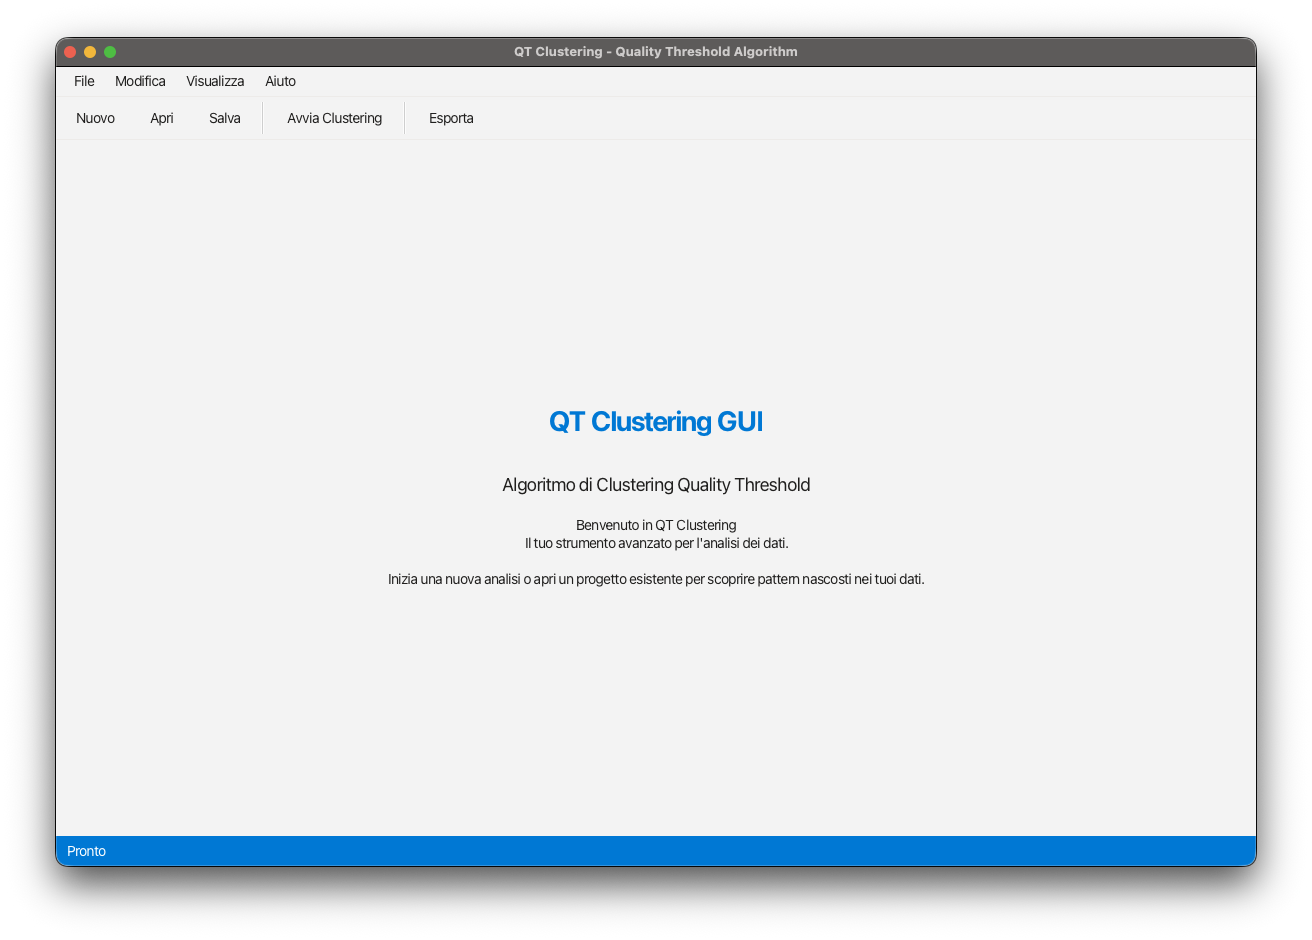
\includegraphics[width=0.95\textwidth]{gui_images/00_Home_Screen.png}
  \caption{Vista generale della GUI all'avvio}
  \label{fig:gui-home-screen}
\end{figure}

La GUI e' organizzata come flusso in tre fasi principali: configurazione iniziale,
esecuzione del clustering e consultazione dei risultati. Questo flusso non e' solo
concettuale, ma e' concretamente implementato nei controller \module{HomeController},
\module{ClusteringController} e \module{ResultsController}, che si scambiano
configurazioni e risultati tramite \module{ApplicationContext}.

\section{Schermata Home: configurazione di una nuova analisi}

\subsection{Selezione della sorgente dati}

La schermata Home permette di scegliere la sorgente dati tra quattro possibilita':
dataset hardcoded \emph{PlayTennis}, dataset standard \emph{Iris}, file CSV e database
MySQL. La scelta effettuata modifica dinamicamente il form: nel caso CSV compare il
selettore di file, mentre nel caso database viene visualizzato il blocco di campi
dedicati a host, porta, nome del database, utente, password e tabella.

Questo comportamento e' gestito da un semplice meccanismo di attivazione e disattivazione
delle sezioni opzionali. Il vantaggio per l'utente e' una riduzione del rumore visivo:
vengono mostrati solo i campi strettamente necessari allo scenario selezionato. Dal punto
di vista documentale, e' importante notare che i valori predefiniti presenti nel form
database sono coerenti con quelli usati nel backend: \module{localhost}, porta 3306,
database \module{MapDB}, utente \module{MapUser} e password \module{map}.

\subsection{Validazione del radius e dei campi obbligatori}

Il parametro \emph{radius} viene inserito nella schermata Home e validato immediatamente.
La GUI impone tre condizioni: il campo non deve essere vuoto, il valore deve essere
numerico e il numero deve appartenere all'intervallo $[0,1]$. L'ultimo vincolo riflette
la distanza normalizzata usata dal backend e aiuta l'utente a restare entro un dominio
semanticamente sensato.

La validazione complessiva del form non riguarda pero' solo il raggio. Nel caso CSV viene
richiesto un file selezionato, mentre nel caso database devono essere presenti almeno
nome database, utente, password e nome tabella. Solo quando l'intera configurazione
risulta coerente la GUI abilita il pulsante \emph{Avvia Clustering}. Questa scelta rende
esplicito che la schermata Home non e' un semplice pannello di preferenze, ma il luogo in
cui viene costruita la configurazione operativa che guidera' il backend.

\subsection{Anteprima del dataset}

Il pulsante \emph{Anteprima Dataset} apre un dialogo modale che mostra una tabella con le
prime righe del dataset e una seconda scheda con statistiche sugli attributi. Nel caso di
attributi continui vengono riportati minimo e massimo; nel caso di attributi discreti
viene mostrato il numero di valori distinti. Questo dialogo e' particolarmente utile
quando si caricano tabelle da database, perche' consente di verificare rapidamente se i
dati letti dal backend corrispondono alle aspettative dell'utente.

Va pero' sottolineata una limitazione concreta dell'implementazione corrente: l'anteprima
da CSV non e' ancora disponibile dalla schermata Home. Se si seleziona un file CSV e si
richiede la preview, l'applicazione segnala esplicitamente che tale funzione non e'
supportata. Il manuale tiene conto di questo comportamento e non lo presenta come una
funzionalita' pienamente disponibile.

\section{Schermata di esecuzione del clustering}

\subsection{Avvio automatico del processo}

Una volta confermata la configurazione, la GUI crea un oggetto
\module{ClusteringConfiguration}, lo memorizza nel contesto applicativo e carica la vista
\module{clustering.fxml}. L'ingresso in questa vista fa partire automaticamente il
processo di elaborazione: non e' necessario premere un ulteriore pulsante per lanciare
l'algoritmo. Questa scelta enfatizza il carattere transitorio della schermata, pensata
non come area di configurazione ma come monitor di esecuzione.

\begin{figure}[H]
  \centering
  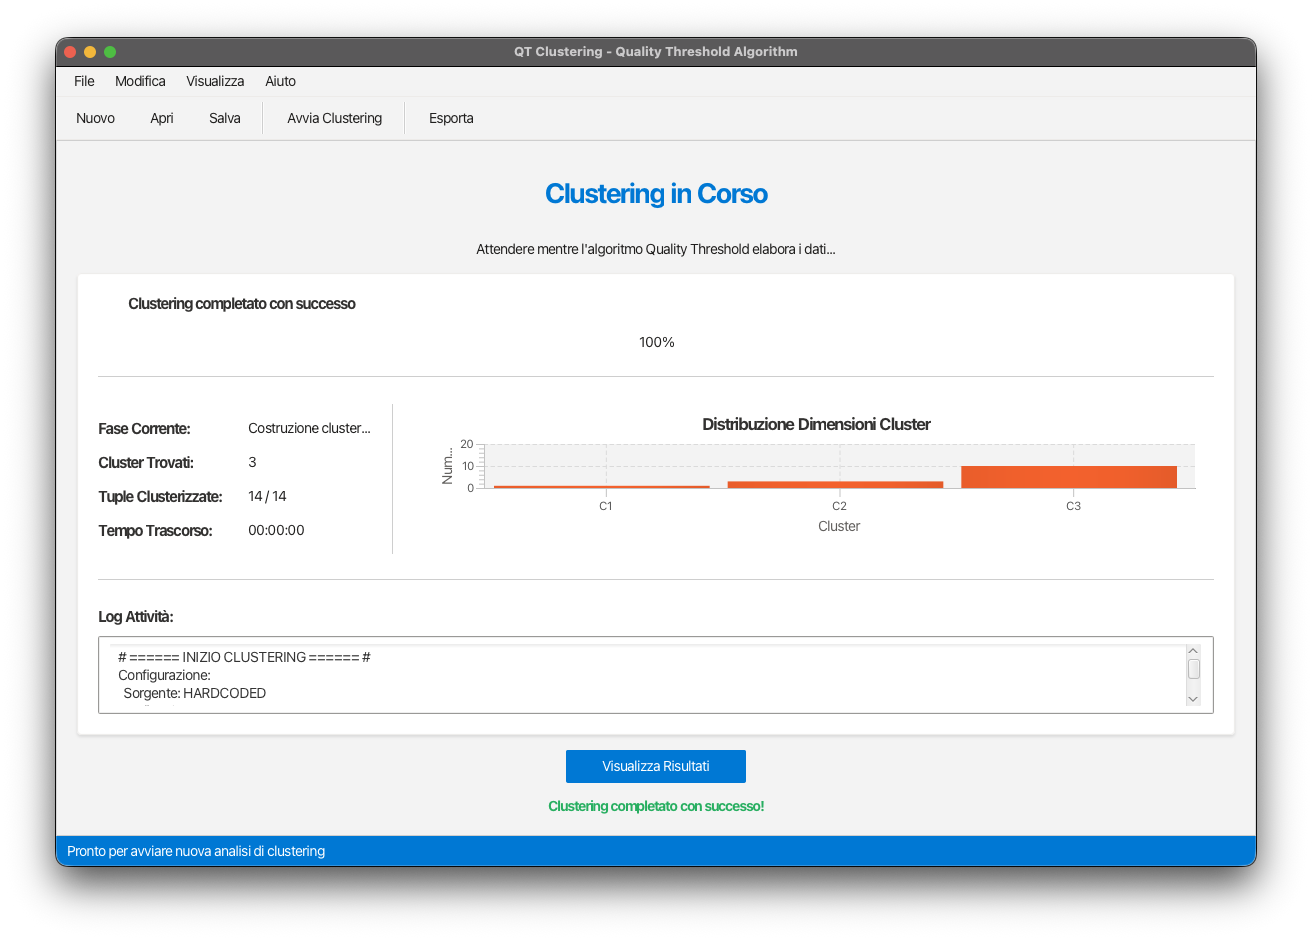
\includegraphics[width=0.95\textwidth]{gui_images/02_Esecuzione_Clustering.png}
  \caption{Schermata di esecuzione con barra di progresso, log e statistiche parziali}
  \label{fig:gui-clustering}
\end{figure}

\subsection{Informazioni mostrate durante l'elaborazione}

La schermata espone quattro gruppi di informazioni. In alto compare una barra di
progresso accompagnata da un indicatore numerico percentuale. Nel pannello laterale
vengono aggiornati la fase corrente, il numero di cluster trovati, il numero di tuple
clusterizzate e il tempo trascorso. Nella parte inferiore una \module{TextArea} raccoglie
il log dell'attivita', documentando caricamento del dataset, avvio dell'algoritmo, numero
di cluster trovati e tempi di esecuzione.

Quando il clustering termina con successo, la vista genera anche un grafico a barre con
la distribuzione delle dimensioni dei cluster. Questo grafico non sostituisce la
successiva visualizzazione dettagliata, ma svolge un ruolo di riepilogo immediato:
permette di capire se il raggio scelto ha prodotto cluster numerosi e pochi, oppure molti
cluster piccoli.

\subsection{Annullamento e gestione degli errori}

La GUI consente di interrompere l'operazione in corso con il pulsante \emph{Annulla
Clustering}. L'azione non e' immediata e silenziosa: viene prima richiesto un consenso
esplicito all'utente, poi il task JavaFX in background viene marcato come annullato e la
vista mostra un messaggio di stato dedicato. In caso di errore, la schermata presenta un
alert modale e aggiorna sia il log sia la zona di stato. L'obiettivo di questa
progettazione e' duplice: evitare chiusure improvvise della vista e lasciare una traccia
leggibile di cio' che e' avvenuto.

\section{Schermata Risultati}

\subsection{Pannello di riepilogo e struttura ad albero}

La vista risultati riassume anzitutto metriche globali: numero di cluster, numero di
tuple, valore del raggio, dimensione media, cluster piu' grande e cluster piu' piccolo.
Sotto questo riepilogo compare una struttura \module{TreeView} in cui ogni cluster e'
presentato come nodo espandibile, contenente a sua volta le tuple appartenenti al
cluster. La struttura ad albero e' coerente con il modello interno del backend, dove ogni
cluster conserva l'elenco ordinato degli identificativi delle tuple che lo compongono.

\begin{figure}[H]
  \centering
  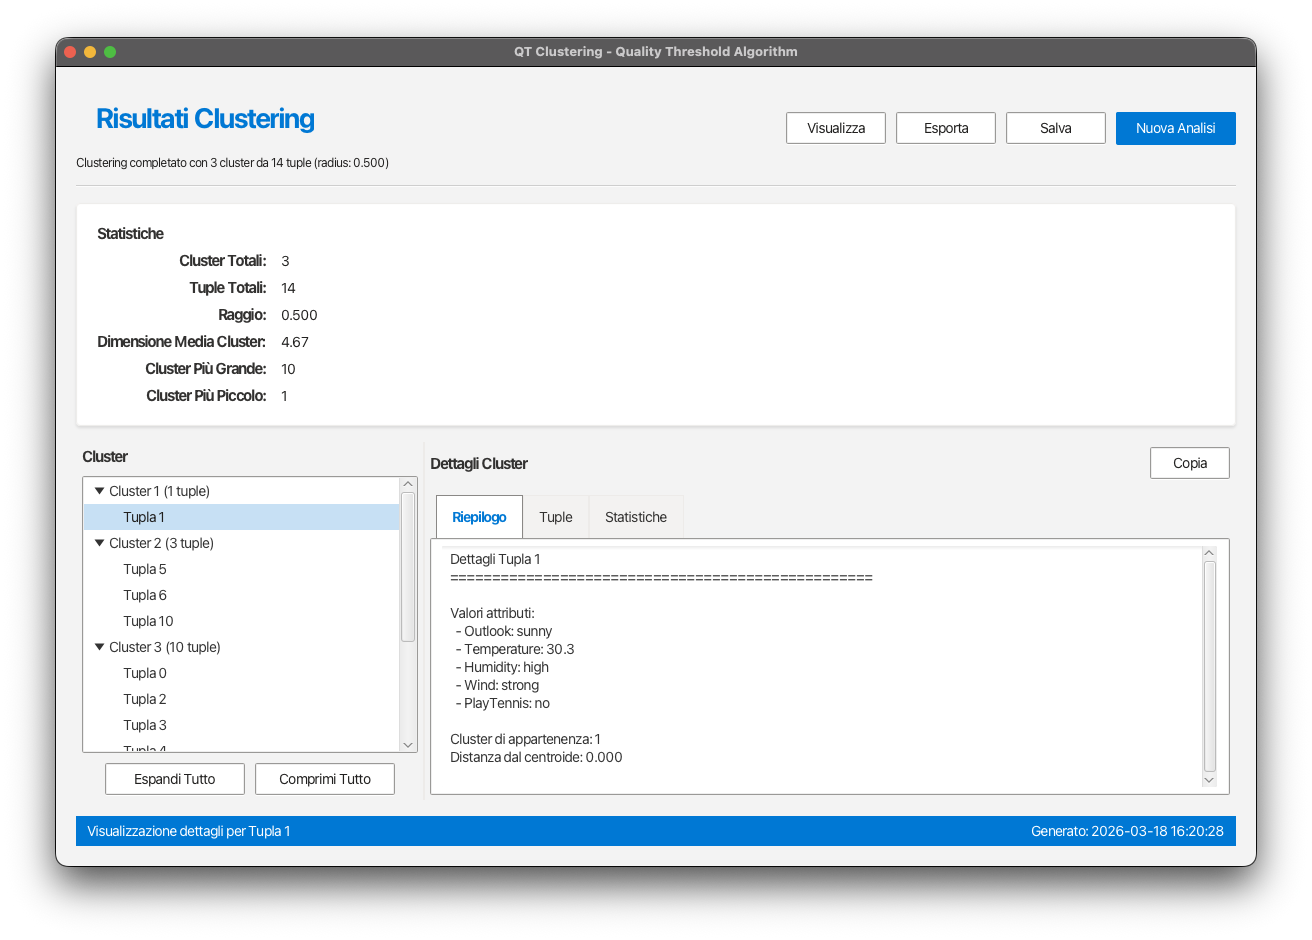
\includegraphics[width=0.95\textwidth]{gui_images/03_Risultati_Clustering.png}
  \caption{Vista risultati con statistiche generali, albero dei cluster e pannelli di dettaglio}
  \label{fig:gui-results}
\end{figure}

\subsection{Pannelli di dettaglio}

La selezione di un cluster popola tre pannelli testuali distinti. Il primo fornisce un
riepilogo testuale del cluster, comprensivo di centroide e distanza media. Il secondo
elenca le tuple del cluster e, per ciascuna, la distanza dal centroide. Il terzo
sintetizza statistiche numeriche come dimensione, distanza minima, massima e media. Se
invece l'utente seleziona una singola tupla dall'albero, la vista mostra i valori degli
attributi e individua il cluster di appartenenza con relativa distanza dal centroide.

Questa tripartizione dei dettagli e' particolarmente utile in chiave didattica. L'utente
puo' infatti passare da una lettura sintetica del cluster a una verifica puntuale dei
suoi elementi senza cambiare schermata o aprire finestre accessorie. Il pulsante
\emph{Copia} permette inoltre di trasferire rapidamente il contenuto corrente negli
appunti del sistema.

\subsection{Statistiche avanzate}

Oltre alla vista principale, la GUI mette a disposizione un dialogo di statistiche
avanzate. Questo dialogo e' articolato in quattro schede: statistiche generali,
distribuzione delle dimensioni dei cluster, distribuzione delle distanze dal centroide e
tabella riepilogativa dei cluster. La distribuzione delle distanze e' costruita come
istogramma su dieci intervalli, mentre la tabella riepilogativa riporta per ogni cluster
dimensione, distanze media/minima/massima e una preview testuale del centroide.

Il dialogo non introduce metriche esterne all'implementazione del backend, ma riorganizza
in modo comparativo informazioni gia' presenti nei risultati. In questo senso costituisce
uno strumento di lettura, non una seconda fase di elaborazione.

\section{Visualizzazione grafica dei cluster}

\subsection{Scelta degli assi e rappresentazione dei punti}

Il pulsante \emph{Visualizza} apre una finestra separata basata su XChart. La finestra
consente di scegliere quale attributo usare per l'asse X e quale per l'asse Y. Se gli
attributi sono continui, i valori vengono riportati direttamente sul piano. Se invece
l'attributo selezionato e' discreto, la GUI costruisce un mapping ordinale stabile tra
valori simbolici e interi, cosi' da poter comunque produrre una visualizzazione 2D
coerente. Questo significa che anche attributi categorici possono essere mostrati sul
grafico, pur richiedendo una interpretazione qualitativa delle coordinate.

\subsection{Modalita' Convex Hull}

Per ogni cluster la vista grafica disegna i punti della serie corrispondente e, se
richiesto, un bordo di \emph{convex hull}. L'inviluppo convesso viene calcolato con
l'algoritmo di Graham Scan e viene mostrato solo se il cluster contiene almeno tre punti;
cluster troppo piccoli non generano quindi alcun bordo. Il rendering attuale privilegia
il contorno e non il riempimento dell'area, scelta dettata dai vincoli della libreria
grafica adottata.

\subsection{Esportazione del grafico}

La finestra di visualizzazione permette di esportare il grafico in PNG in due formati:
standard da 800$\times$600 pixel e alta definizione da 1920$\times$1080 pixel. La
funzione non salva una schermata della finestra, ma rigenera il grafico con le dimensioni
richieste e lo scrive su file. In questo modo il PNG prodotto resta nitido anche quando
viene usato in report esterni o presentazioni.

\section{Persistenza ed esportazione dalla GUI}

La GUI distingue nettamente tra \emph{salvataggio} ed \emph{esportazione}. Il salvataggio
produce un file \module{.dmp} tramite serializzazione completa del clustering, del
dataset e del \emph{radius}; l'operazione e' accessibile dal menu \emph{File} o dalla
toolbar. L'apertura di un file \module{.dmp} riporta invece l'utente direttamente alla
schermata risultati, a condizione che il file contenga il dataset oltre ai cluster.

L'esportazione, accessibile dalla schermata risultati, offre tre formati: CSV, report
testuale TXT e archivio ZIP. Il CSV e' orientato all'analisi tabellare, il TXT alla
consultazione testuale e il ZIP alla distribuzione di un pacchetto completo comprendente
\module{.dmp}, CSV, report e un breve \module{README.txt} interno.

\section{Schermata Impostazioni}

La schermata \emph{Impostazioni} raccoglie preferenze di aspetto, parametri predefiniti
di clustering, opzioni di esportazione e configurazione database. Il
\module{ThemeManager} applica in tempo reale il cambio di tema e la variazione della
dimensione dei font, mentre il controller salva il resto delle preferenze nel file
\filepath{qtgui.properties}.

\begin{figure}[H]
  \centering
  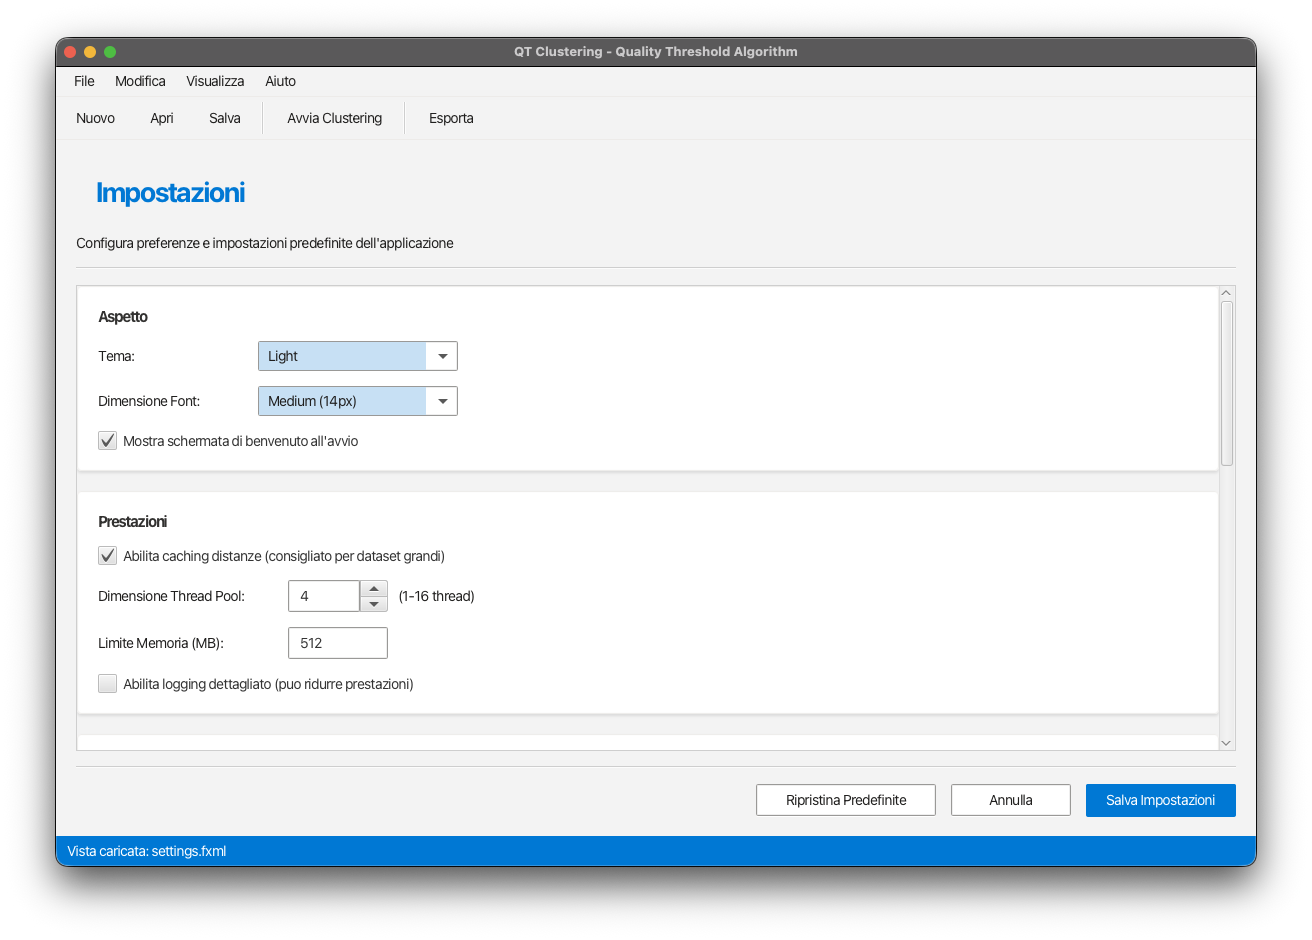
\includegraphics[width=0.9\textwidth]{gui_images/07.1_Impostazioni.png}
  \caption{Schermata delle impostazioni dell'applicazione}
  \label{fig:gui-settings}
\end{figure}

Dal punto di vista pratico, le impostazioni piu' rilevanti sono la cartella di
esportazione, i parametri di connessione al database e i valori predefiniti come il
\emph{radius}. La schermata include inoltre un pulsante per testare la connessione JDBC
in background, mostrando un alert di successo o fallimento. L'utente deve pero' tenere
presente che il dialogo di export effettivamente usato nella schermata risultati offre i
formati realmente supportati dall'applicazione, cioe' CSV, TXT e ZIP per i risultati e
PNG per i grafici.
